\documentclass[10pt,a4j]{article}

\def\Vec#1{\mbox{\boldmath $#1$}}
\usepackage[dvipdfmx]{graphicx}

\setlength{\textheight}{275mm}
\headheight 5mm
\topmargin -20mm
\textwidth 160mm
\textheight 250mm
\oddsidemargin -0mm
\evensidemargin -5mm

\pagestyle{empty}
\makeatletter
  \def\@maketitle{%
  \newpage\null
  \vskip 2em%
  \begin{center}%
  \let\footnote\thanks
    {\large\bf \@title \par}%
    \vskip 1.5em%
    {\large\bf \@author \par}%
    \vskip 1.5em%
    {\small \@date}%
  \end{center}%
}
\makeatother

%\documentclass[10pt, a4j]{article}
%%\usepackage{citesort}
\usepackage{amssymb}
\usepackage[dvipdfmx]{graphicx}% 図を入れるときに使用
\usepackage{wrapfig}% 図の周りに本文を流し込みたいときに使用
\usepackage{subfigure}
\usepackage{here}
\begin{document}
\section{Mg-LPSO合金の第一原理計算による検証}
\subsection{動機}
LPSO 構造の生成機構について,我々は「積層欠陥部にL12\_Clusterが形成され,そこから排斥されたZn, Y が,濃化して新たな積層欠陥を誘発する」というシナリオを立てていた.しかし,清原らの計算ではZn,Yはクラスターからの距離が離れるにつれてより安定するということが示唆されていた.

そこで,自分の研究では排斥されるZn,Yを単一原子,あるいはZn-Yペアのような小さな組織ではなく,Small\_Clusterというもう少し大きな組織として考える事にした.Small\_ClusterとL12\_Cluster間の相互作用について,第一原理計算による検証をおこない,Zn-YがSmall\_Cluster単位で拡散する可能性について考察する.

\subsection{Small\_Clusterに関する検証}
清原らは,hcp構造に強引にL12\_Clusterを導入すると半分の大きさであるSmall\_Clusterに分離すると報告しており,このサイズは奥田らが実験結果として報告しているクラスターサイズに近い.

まずは,L12\_Clusterがどのように分離するのかを確かめるために,以下の図のような垂直方向に分割したモデルと平行方向に分割したモデルを用意した.それぞれのモデルを6層のMg結晶に導入し,VASPによる第一原理計算により系全体のエネルギーを算出し比較をおこなった.

\begin{figure}[htbp]\begin{center}
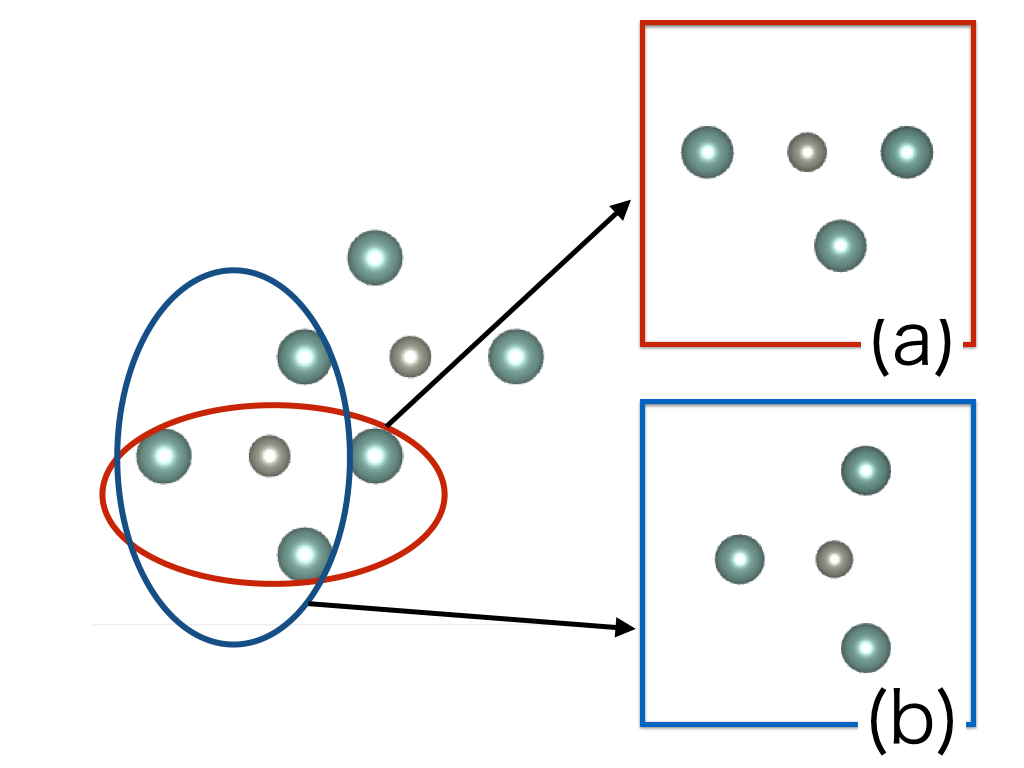
\includegraphics[width=6cm,bb=0 0 442 500]{../figs/./MiniCluster.png}
\caption{}
\label{default}\end{center}\end{figure}
結果は垂直方向に分割したモデルの方が0.2eVほど安定しており,本研究ではこのZn-Yの集合をSmall\_Clusterとして扱う事とした,

\subsection{Small\_ClusterとL12\_Cluster間の相互作用}
Small\_ClusterがL12\_Clusterと垂直方向でどのような距離をとった時に安定するのかを検証するために,18層のスラブモデルにL12\_ClusterとSmall\_Clusterを挿入し計算をおこなった.VASPによる計算では周期的境界条件を使用しているため,想定しているL12\_Clusterではない,上部のL12\_Clusterからの影響も考慮しなければならない.そこで,18層のモデルでの計算では影響を受けない範囲として,L12\_Clusterから7層離れた位置までにそれぞれSmall\_Clusterを配置し計算をおこなった.Small\_Clusterの平行方向の座標については,L12\_Clusterの真上の位置にSmall\_Clusterを配置した.

\begin{figure}[htbp]\begin{center}
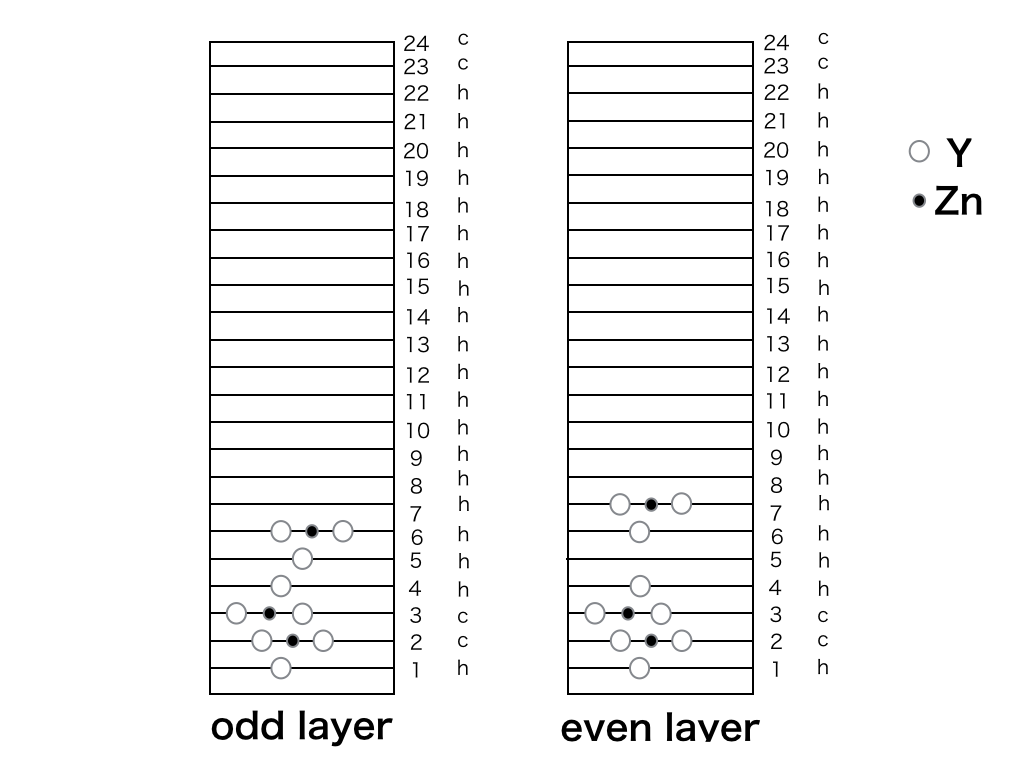
\includegraphics[width=6cm,bb=0 0 442 500]{../figs/./small_cluster_slab.png}
\caption{}
\label{default}\end{center}\end{figure}
この計算では,4層での計算結果が収束しなかったが,他の層の計算結果を見るに僅かではあるが中距離での安定を示す結果となった.しかし,結果が出ていない8層以降の層において単調増加を示した場合には上部のクラスターからの影響を受けてエネルギーが増加しているだけ,という考察となる.

\begin{figure}[htbp]\begin{center}
\includegraphics[width=6cm,bb=0 0 442 500]{../figs/./small_cluster_18.png}
\caption{}
\label{default}\end{center}\end{figure}
5層から7層にかけてのエネルギーの増大が中距離安定を示すのかを確かめるために,更に層数を増やした24層のスラブモデルでの計算をおこなった,このモデルでは10層離れた位置までにそれぞれSmall\_Clusterを配置し計算をおこなった.この計算結果からは,7層までは18層での計算と同様のエネルギー傾向が見られ,更に8層から10層にかけてはエネルギー増減なしという結果が得られた.この結果はSmall\_Clusterが中距離で安定するという仮説を支持している.

\begin{figure}[htbp]\begin{center}
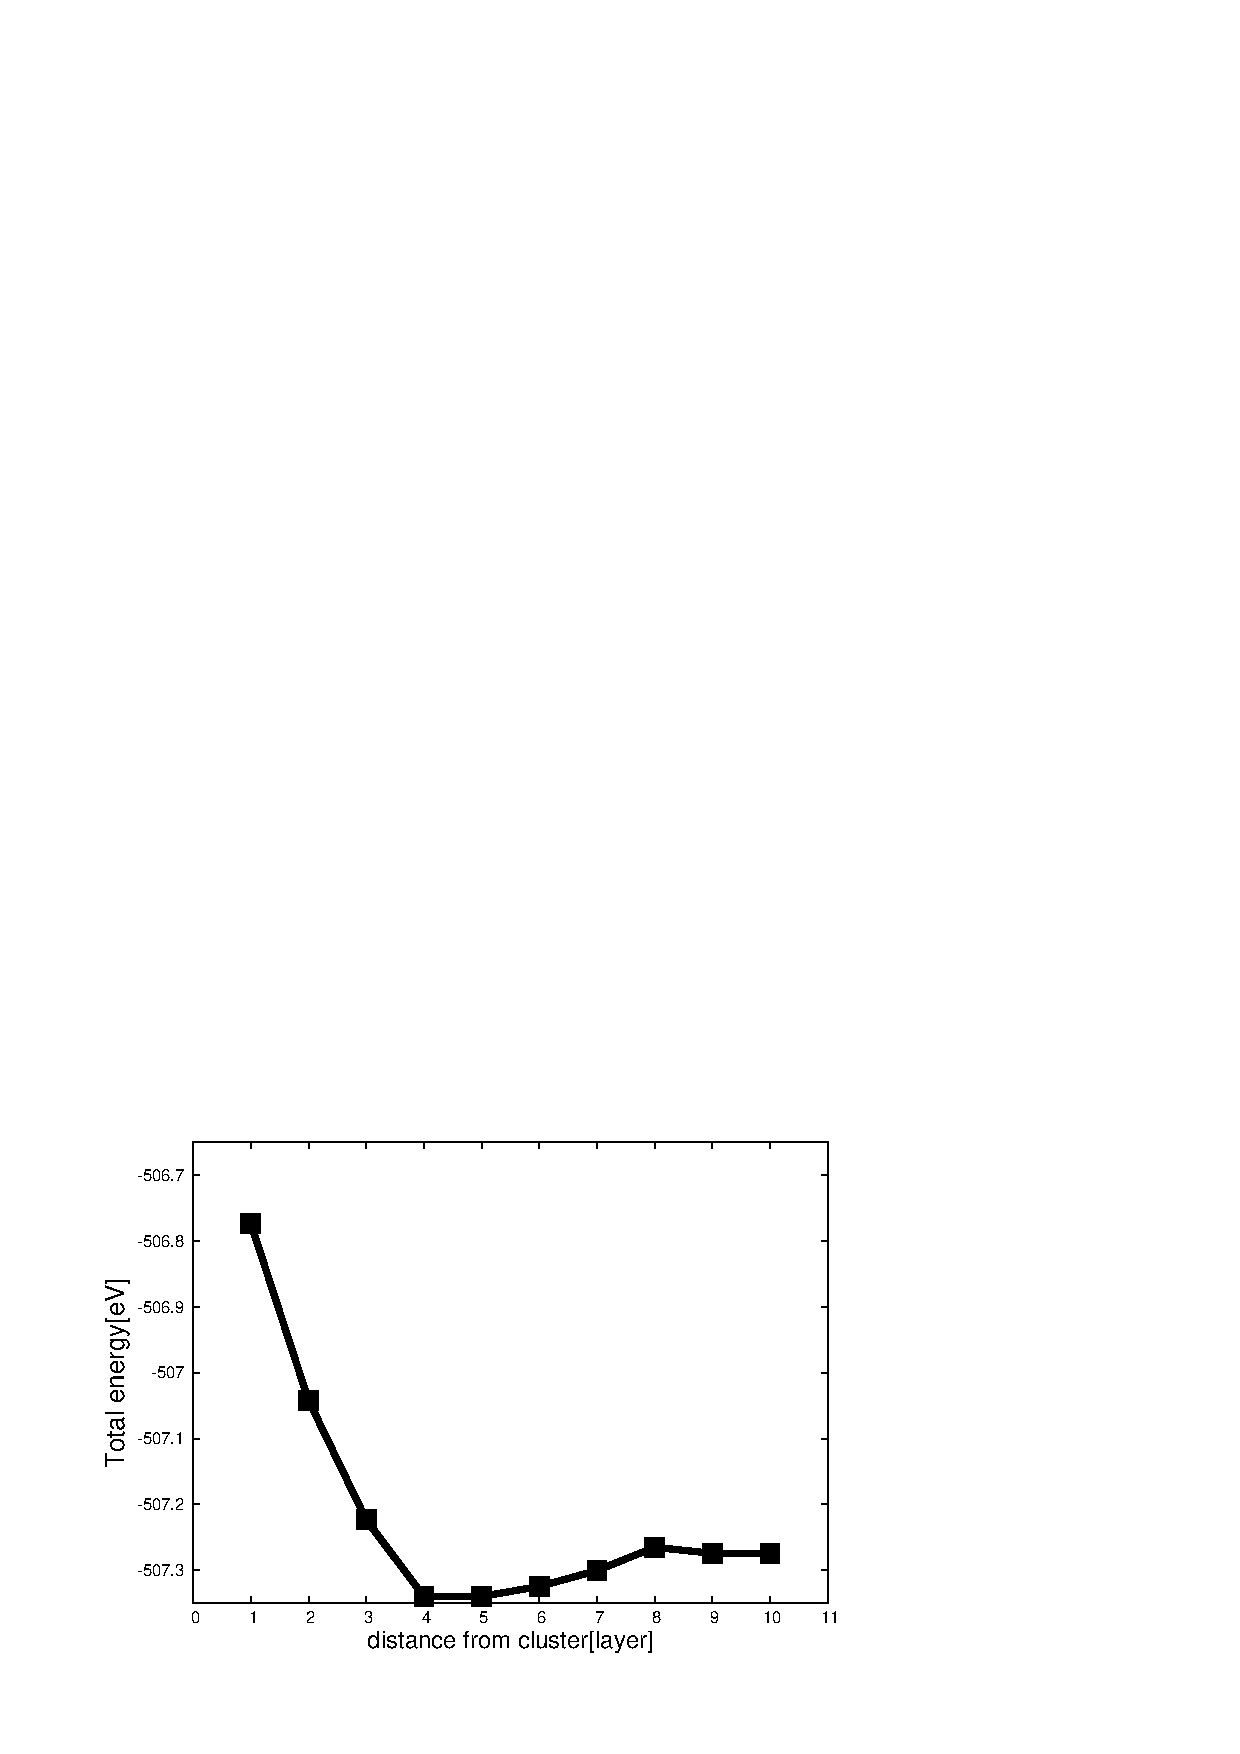
\includegraphics[width=6cm,bb=0 0 442 500]{../figs/./small_cluster_24.png}
\caption{}
\label{default}\end{center}\end{figure}
Small\_ClusterとL12\_Cluster間の距離によって上記のエネルギー傾向に違いが出るのかを確かめるために,久保らがまとめたL12\_Clusterの近接距離の図を参考にそれぞれの近接距離にSmall\_Clusterの頂点を配置したモデルについて計算をおこなった.この計算でSmall\_Clusterを平行方向にずらしても同様のエネルギー傾向を示すことがわかった.

\begin{figure}[htbp]\begin{center}
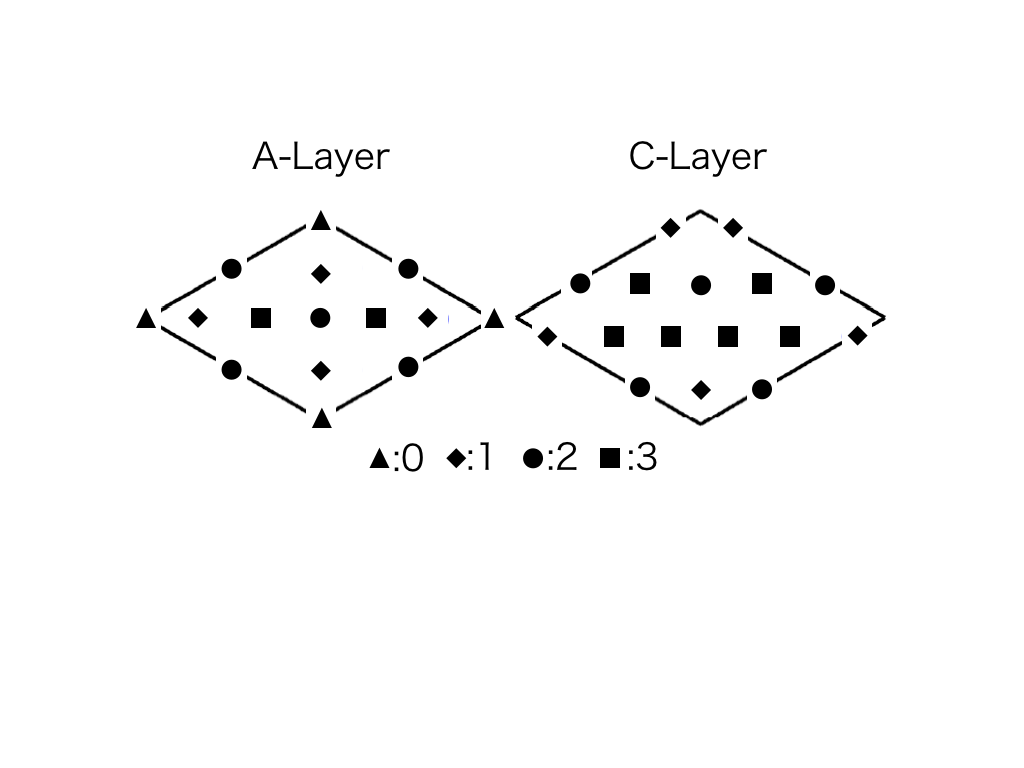
\includegraphics[width=6cm,bb=0 0 442 500]{../figs/./distance_from_cluster.png}
\caption{}
\label{default}\end{center}\end{figure}
\begin{figure}[htbp]\begin{center}
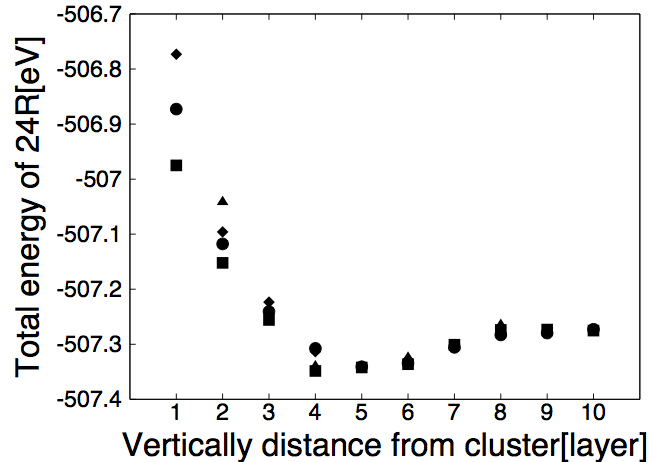
\includegraphics[width=6cm,bb=0 0 442 500]{../figs/./small_cluster_Alld.png}
\caption{}
\label{default}\end{center}\end{figure}
以上の計算結果から,我々は積層欠陥部にL12\_Clusterが形成され,そこから排斥されたZn, Y が中距離でsmall\_clusterとして安定し,濃化して新たな積層欠陥を誘発する」という仮説を立てている.

\subsection{クラスター拡散}
ここまでで溶質原子の中距離での安定を示したが,溶質原子が排斥された後の拡散法については解明されていない.ここでSmall\_Clusterがクラスター単位で拡散するのではないか,という仮説を立てて第一原理計算をおこなっている.

まず,Mg結晶において拡散に必要となる空孔が用意に形成されるのかどうかを検証するため,Mg結晶中で空孔が形成されるためのエネルギーを計算した.計算結果,空孔の形成エネルギーは-0.7552799eVという結果を示した.この値は小さいとはいえず,Mg結晶中で空孔が形成されやすいという事を支持しない結果となった.

次にSmall\_Clusterの近くで空孔が安定するか,という事を検証するために,Small\_Clusterから近い位置,遠い位置にそれぞれ空孔を配置し第一原理計算をおこなった.この結果は遠い位置に空孔がある方が安定という結果を示し,仮説を支持しない結果となった.
\end{document}
